% =============================================================================
% bo-convergence.tex — Bayesian optimization convergence plot with error bars
%
% Shows: best-observed-value vs. iteration for two methods, with small
% vertical error-bar ticks at each point. Hand-drawn axes (no pgfplots
% dependency — matches the plain-TikZ convention used by regression-scatter.tex).
% Compiles standalone via: xelatex bo-convergence.tex
% =============================================================================

\documentclass[border=4pt]{standalone}
\usepackage{tikz}
\usetikzlibrary{arrows.meta}

\definecolor{method}{HTML}{012169}
\definecolor{baseline}{HTML}{6B7280}
\definecolor{axis}{HTML}{1A1A1A}

% -----------------------------------------------------------------------------
% Diagram: x-axis is iteration count on an uneven grid (x-position i maps to
%   iteration label at that tick, not a literal linear count — the common
%   convergence-plot convention for early-dense/late-sparse logging).
% Iteration labels at x = 0..6: 1, 5, 10, 20, 30, 40, 50.
% y-coordinates are the raw "best observed value" (0-100 score) divided by 8
%   so a 45-unit data range (55-100) doesn't stretch into a 45cm-tall figure
%   at TikZ's 1cm/unit default — tick LABELS still print the real value.
%   (Deliberately pre-dividing the coordinates, not a tikzpicture `scale=`,
%   since a bare scale is banned by prevention rule P3.)
% "Our Method" y-values (solid, navy circle): 68, 85, 91, 94, 95.5, 96, 96.3
%   error half-width: 1.5 at every point (also /8 in the drawn coordinates).
% "Baseline" y-values (dashed, gray square): 60, 74, 82, 86, 88, 89.5, 90.5
%   error half-width: 2.0 at every point (also /8 in the drawn coordinates).
% -----------------------------------------------------------------------------

\begin{document}
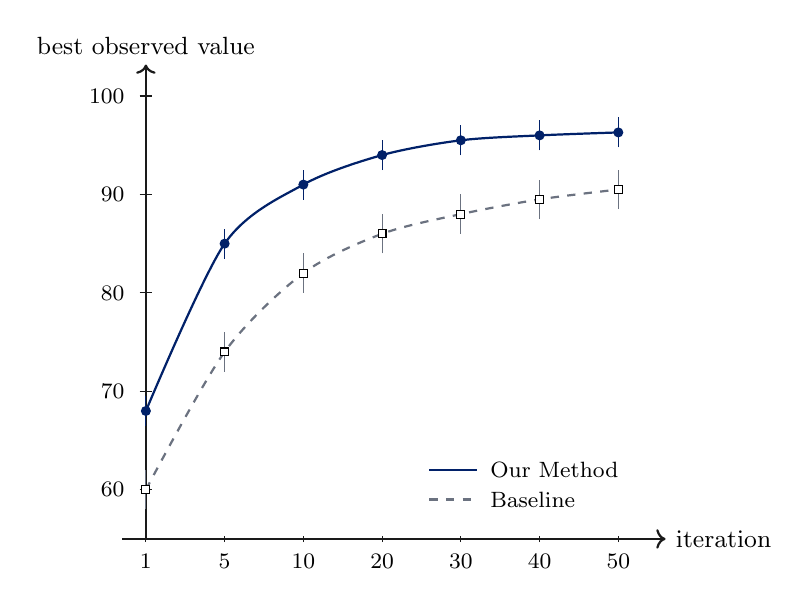
\begin{tikzpicture}
  % Axes (55/8 = 6.875 origin, 100/8 = 12.5 top plus headroom)
  \draw[->, thick, draw=axis] (-0.3, 6.875) -- (6.6, 6.875) node[right] {\small iteration};
  \draw[->, thick, draw=axis] (0, 6.875) -- (0, 12.9) node[above] {\small best observed value};

  % X ticks with the actual (uneven-grid) iteration labels
  \foreach \x/\lab in {0/1, 1/5, 2/10, 3/20, 4/30, 5/40, 6/50} {
    \draw[draw=axis] (\x, 6.835) -- (\x, 6.915);
    \node[below, font=\footnotesize] at (\x, 6.8) {\lab};
  }
  \foreach \y in {60, 70, 80, 90, 100} {
    \draw[draw=axis] (-0.08, \y/8) -- (0.08, \y/8);
    \node[left, font=\footnotesize] at (-0.15, \y/8) {\y};
  }

  % Error bars — draw first so the curves and markers sit on top
  \foreach \x/\y in {0/68, 1/85, 2/91, 3/94, 4/95.5, 5/96, 6/96.3}
    \draw[draw=method] (\x, \y/8-0.19) -- (\x, \y/8+0.19);
  \foreach \x/\y in {0/60, 1/74, 2/82, 3/86, 4/88, 5/89.5, 6/90.5}
    \draw[draw=baseline] (\x, \y/8-0.25) -- (\x, \y/8+0.25);

  % Curves
  \draw[thick, draw=method] plot[smooth] coordinates {
    (0,68/8) (1,85/8) (2,91/8) (3,94/8) (4,95.5/8) (5,96/8) (6,96.3/8)
  };
  \draw[thick, dashed, draw=baseline] plot[smooth] coordinates {
    (0,60/8) (1,74/8) (2,82/8) (3,86/8) (4,88/8) (5,89.5/8) (6,90.5/8)
  };

  % Markers
  \foreach \x/\y in {0/68, 1/85, 2/91, 3/94, 4/95.5, 5/96, 6/96.3}
    \filldraw[method] (\x, \y/8) circle (1.6pt);
  \foreach \x/\y in {0/60, 1/74, 2/82, 3/86, 4/88, 5/89.5, 6/90.5}
    \draw[baseline, fill=white] (\x-0.05, \y/8-0.05) rectangle (\x+0.05, \y/8+0.05);

  % Legend — placed in the empty lower-right corner, clear of both curves
  \draw[thick, draw=method] (3.6, 7.75) -- (4.2, 7.75);
  \node[right, font=\footnotesize] at (4.25, 7.75) {Our Method};
  \draw[thick, dashed, draw=baseline] (3.6, 7.375) -- (4.2, 7.375);
  \node[right, font=\footnotesize] at (4.25, 7.375) {Baseline};
\end{tikzpicture}
\end{document}
